\adparagraph{Kendall Tau Distance}
Looking at Figure \ref{fig:kendalldistance} we can see the results of the KTD test. As covered in Section \ref{sec:distance} the distance measures have a score between 0 and 1 where 0 correspond to equal lists, 1 is that the lists are reverse of each other, and 0.78 is that the lists are disjoint as we used an average approach.

Looking at the approaches individually Avg clearly scores the highest. The reason is that Avg disregards the item ranks in the top-k lists and aggregates them based on the average rating between the group members instead. SF performs worse than both \MC and BC, which could be seen as having to do with SF ranking its candidates using a median like approach, which is closer to how Avg performs. Lastly, performing best and almost equal we have BC and \MC. Worth noting is that when the groups are small \MC performers slightly better than BC, but already at group size 8 BC out scales \MC.


\begin{figure}[H]
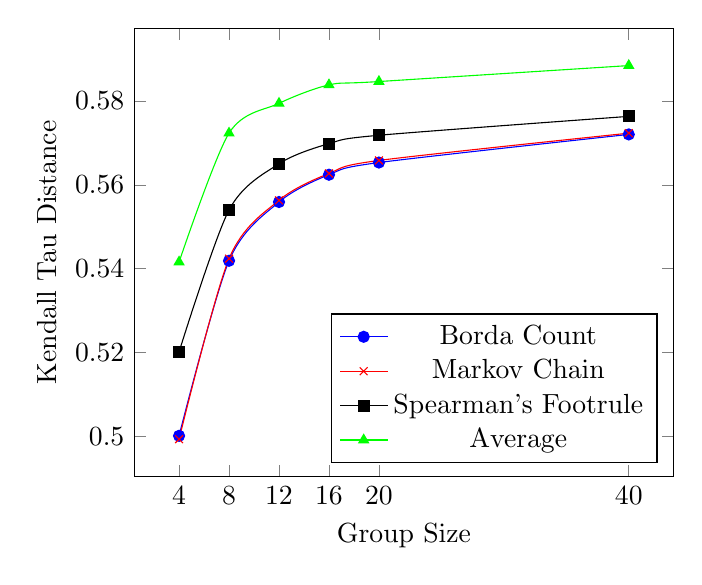
\begin{tikzpicture}
    \begin{axis}[
        xlabel=Group Size,
        ylabel=Kendall Tau Distance,
        xtick = {4,8,12,16,20,40},
        legend pos=south east]
    \addplot[smooth,mark=*,blue] plot coordinates {
        (4,0.5002)
        (8,0.5419)
        (12,0.5559)
        (16,0.5624)
        (20,0.5653)
        (40,0.572)
    };
    \addlegendentry{Borda Count}

    \addplot[smooth,color=red,mark=x] plot coordinates {
            (4,0.4994)
            (8,0.5424)
            (12,0.5563)
            (16,0.5627)
            (20,0.5658)
            (40,0.5723)
        };
    \addlegendentry{Markov Chain}
    
        \addplot[smooth,color=black,mark=square*] plot coordinates {
            (4,0.5202)
            (8,0.554)
            (12,0.565)
            (16,0.5698)
            (20,0.5718)
            (40,0.5763)
        };
    \addlegendentry{Spearman's Footrule}
    
    \addplot[smooth,color=green,mark=triangle*] plot coordinates {
            (4,0.5416)
            (8,0.5723)
            (12,0.5794)
            (16,0.5838)
            (20,0.5846)
            (40,0.5884)
        };
    \addlegendentry{Average}
    
    \end{axis}
\end{tikzpicture}
\caption{Results using KDT} \label{fig:kendalldistance}
\end{figure}
\newpage
When looking at the percentage distance increase between group sizes in Table \ref{tbl:kendall}, it can be seen that all the methods follow the same trend across the group sizes. There is a large difference with an average increase of $7.28$ percent between group sizes 4 and 8, as the groups grow the increase in the KTD quickly fades and becomes very low between groups. By the time we reach groups 20 and 40 the average change in distance is only $0.945$ percent.

For the t-tests shown in Table \ref{tbl:ktd_ttest}, all results are shown to be statistically significant in their differences, except for one case between BC and MC. The remainder are different enough to be statistically significant, but the p-values are still considerably higher than usual between BC and MC for a sample of this size.
\begin{table}[H]
	\centering
	\begin{tabular}{|l|lllll|}\hline
		& 4 to 8 & 8 to 12 & 12 to 16 & 16 to 20 & 20 to 40 \\\hline
		BC 	& 8.34	& 2.58	& 1.17  & 0.52	& 1.19 \\
		MC  & 8.61 	& 2.56	& 1.15	& 0.55	& 1.15 \\
		SF  & 6.50	& 1.99	& 0.85	& 0.35	& 0.79 \\
		Avg	& 5.67	& 1.24 	& 0.76	& 0.14	& 0.65 \\ \hline
	\end{tabular}
	\caption{Percentage increase between the groups for KDT}
	\label{tbl:kendall}
\end{table}


\begin{table}[H]
	\centering
	\begin{tabular}{|l|llllll|}\hline
		& 4 & 8 & 12 & 16 & 20 & 40 \\\hline
		BC/MC	& $0.038$	& $0.031$	& $0.02$	& \textbf{0.071}	& $9e^{-5}$	& $0.002$ \\
		BC/SF	& $2e^{-201}$	& $1e^{-231}$	& $1e^{-236}$	& $7e^{-226}$ & $5e^{-227}$ & $1e^{-198}$ \\
		BC/Avg	& $3e^{-276}$	& $4e^{-296}$ 	& $3e^{-305}$	& $9e^{-303}$	& 0 & 0 \\
		MC/SF	& $2e^{-230}$	& $8e^{-239}$ 	& $6e^{-239}$	& $7e^{-239}$	& $2e^{-226}$ & $4e^{-216}$ \\
		MC/Avg	& $4e^{-259}$	& $2e^{-283}$ 	& $7e^{-298}$	& $7e^{-303}$ & $4e^{-321}$ & 0 \\
		SF/Avg	& $1e^{-93}$	& $1e^{-143}$ 	& $5e^{-159}$	& $2e^{-177}$	& $3e^{-199}$ & $3e^{-261}$ \\ \hline
	\end{tabular}
	\caption{P-values for KTD t-test}
	\label{tbl:ktd_ttest}
\end{table}